% -%-%-%-%-%-%-%-%-%-%-%-%-%-%-%-%-%-%-%-%-%-%-%-%-%
% Planning Poker                                   %  
% 10/03/2013                                       %
% -%-%-%-%-%-%-%-%-%-%-%-%-%-%-%-%-%-%-%-%-%-%-%-%-%
\documentclass[dvips,11pt,xcolor=dvipsnames]{beamer}

%%% fontes %%%
\usepackage[english]{babel}
\usepackage[T1]{fontenc}
\usepackage[utf8]{inputenc}   
\usepackage{ae,aecompl,aeguill}  
\usepackage{calligra}

%%% matematicos %%%
\usepackage{amsmath}
\usepackage{amssymb}
\usepackage{mathptmx}

%%% figuras %%%
\usepackage{graphicx}
\usepackage{wrapfig}

%%% tabelas %%%
\usepackage{colortbl}
\usepackage{array}
\usepackage{longtable}
\usepackage{fancyvrb}
\usepackage{color}

%%% outros %%%
\usepackage{url}
\usepackage{breakurl} 
\usepackage{textcomp}
\usepackage{hyperref} %internal links
\usepackage{color}       
\usepackage{indentfirst} %retira padrao americano de paragrafos
\usepackage{multicol}    
\numberwithin{table}{section}
\numberwithin{figure}{section} %numercao de figuras por secao

%%% extras %%%
\RequirePackage{marvosym} % figuras \Letter \Email 
\usepackage{fancyhdr}     % Headers
\usepackage{epsf}
\usepackage{tikz}
\usetikzlibrary{arrows}
\tikzstyle{block}=[draw opacity=0.7,line width=1.4cm]

%%% Beamer style %%%
\usetheme{Warsaw}

% fontes em negrito
\usefonttheme[onlylarge]{structurebold}

% define tamanhos de letras
\setbeamerfont*{frametitle}{size=\normalsize,series=\bfseries}
\setbeamertemplate{navigation symbols}{}% barra de navegacao superior

% \setbeamercovered{transparent}

% -%-%-%-%-%-%-%-%-%
% Inicio Slides  %
% -%-%-%-%-%-%-%-%-%

\title{Poker Planning}                               

\subtitle{An approach to agile estimating} 
\author[Tiago C. Siva]{
  Tiago Chedraoui Silva \\
}
\institute{Télécom Paristech}

\date{March 18, 2013}

\begin{document}

\begin{frame}
  \titlepage
\end{frame}

\begin{frame}{Outline}
  \tableofcontents
\end{frame}


\section{Introduction}

\begin{frame}{Estimation}

  \begin{block}{Objective}
    \begin{itemize}
      
    \item Answering the combined scope/schedule/ressources question for a new product

    \end{itemize}
  \end{block}
  
  \begin{block}{Facts}
    \begin{itemize}
      
    \item Nearly {\color{orange}$\frac{2}{3}$} of projects significantly overrun their cost estimates.
    \item  {\color{orange}64\%} of the features included in products are rarely or never used
    \item The average project exceeds its schedule by  {\color{orange}100\%}
      
    \end{itemize}
  \end{block}
  
  \pause \begin{alertblock}{Conclusion}
    \begin{itemize}
      
    \item Software estimation is hard!
      
    \end{itemize}
  \end{alertblock}

\end{frame}

\section{Planning Poker}

\subsection{Overview}

\begin{frame}{Planning Poker}
  
  \begin{block}{What is it?}
    \begin{itemize}
    \item A consensus-based technique for estimating, mostly used to estimate effort or relative size of user stories commonly in software development.
    %\item  It is most commonly used in agile software development, in particular the Extreme Programming methodology.
    \end{itemize}
  \end{block}

  \begin{exampleblock}{Why use it?}
    \begin{itemize}
   % \item ``The best way I’ve found for agile teams to estimate is by playing planning poker'' (Grenning 2002)
    \item Make the meetings more short and productive, by making them more fun and dynamic.
    \item Results in better estimations than other techniques.
    \end{itemize}
  \end{exampleblock}

\end{frame}

\subsection{Preparing for the meeting}

\begin{frame}{Preparing for the meeting}

  \begin{alertblock}{Participants of a session}

    \begin{itemize}
    \item All of the developers on the team (programmers, testers, database engineers, analysts, user interaction designers)
    \item Product owner
    \end{itemize}
  \end{alertblock}
  
  \begin{exampleblock}{Material - A deck of cards}

\def \scale{0.04}
    \begin{figure}
      \begin{centering}
        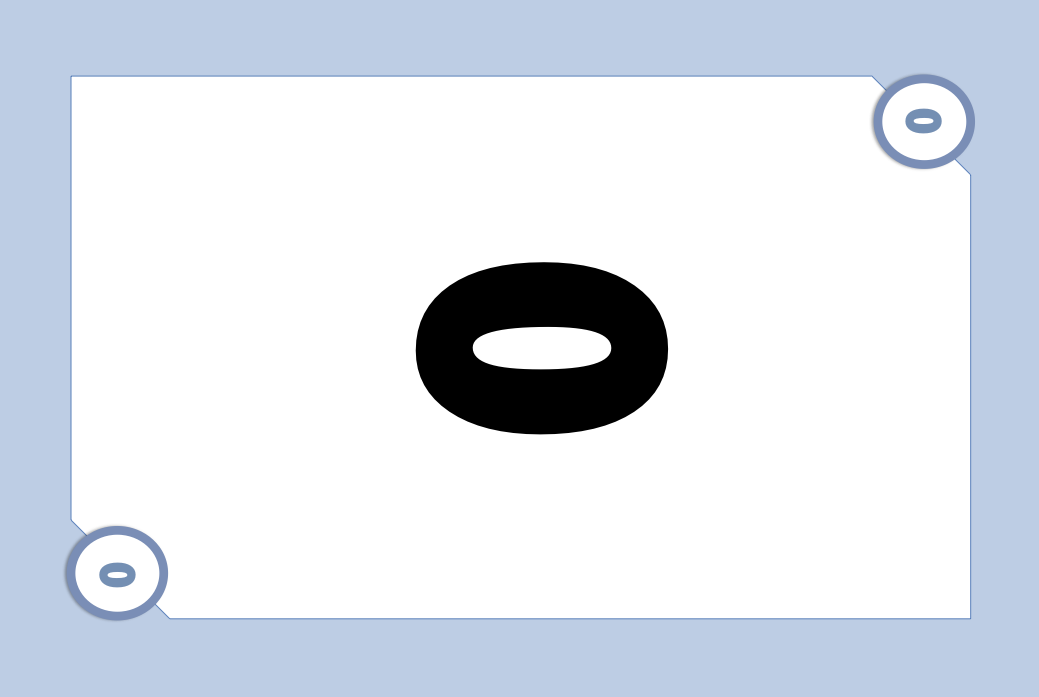
\includegraphics[angle=90,scale=\scale]{img/side-A/b-0}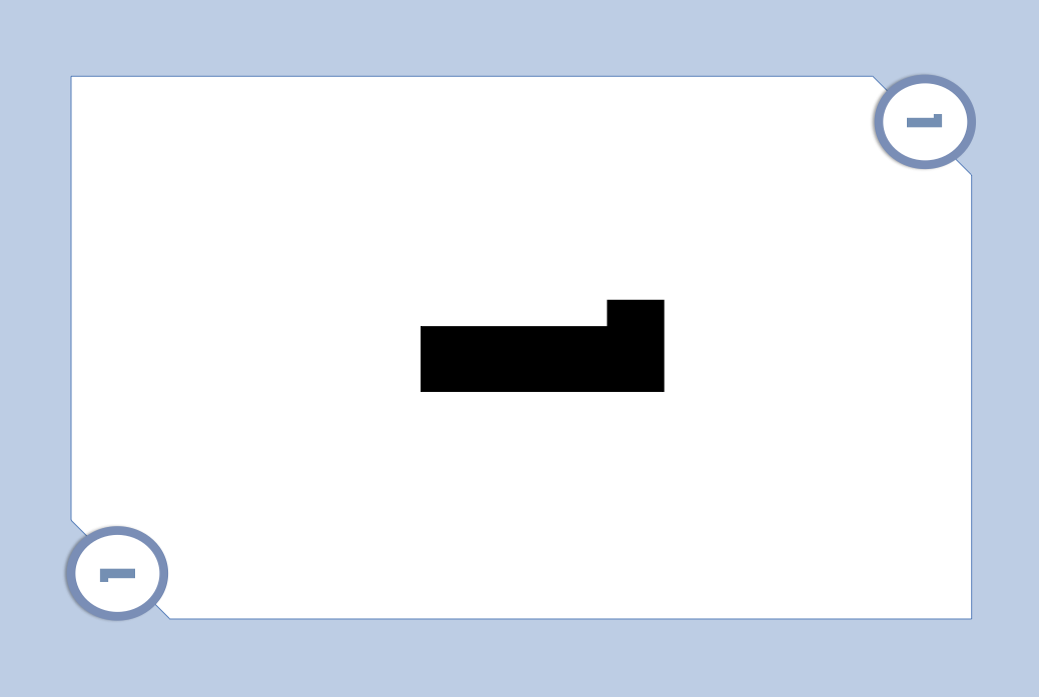
\includegraphics[angle=90,scale=\scale]{img/side-A/b-1}
\includegraphics[angle=90,scale=\scale]{img/side-A/b-2}
\includegraphics[angle=90,scale=\scale]{img/side-A/b-3}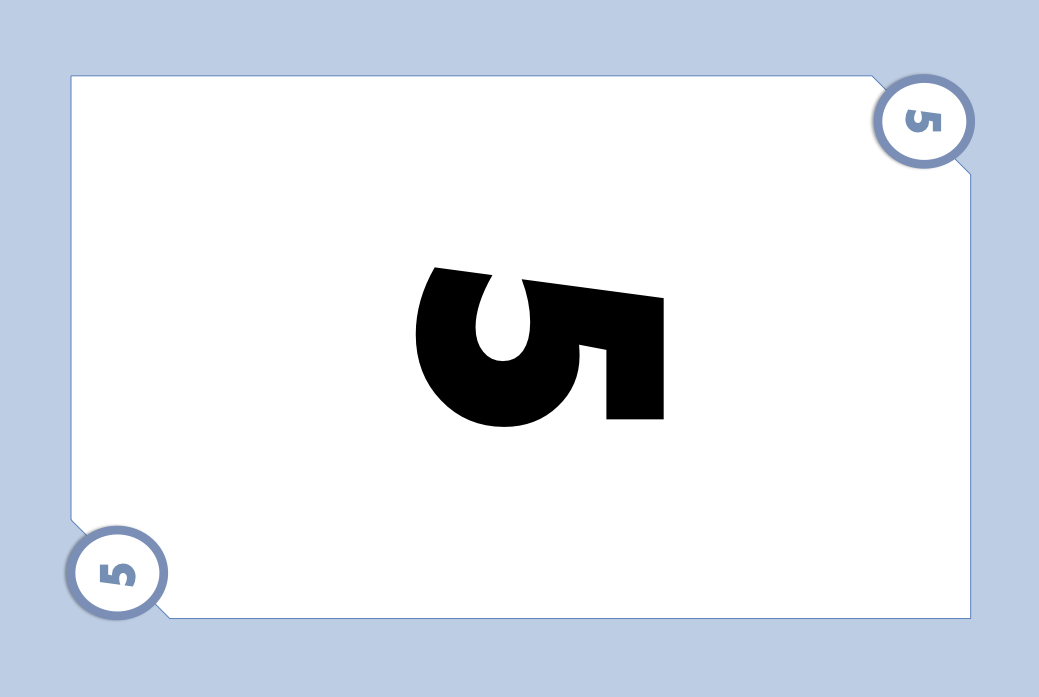
\includegraphics[angle=90,scale=\scale]{img/side-A/b-5}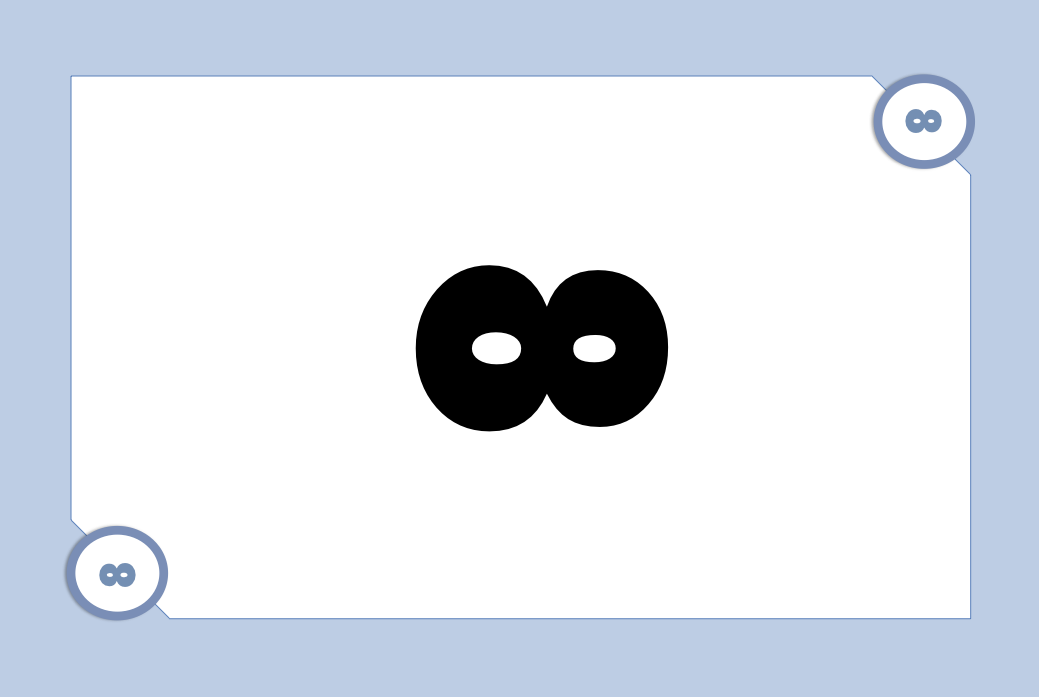
\includegraphics[angle=90,scale=\scale]{img/side-A/b-8}
        \par\end{centering}
      
      \begin{centering}
        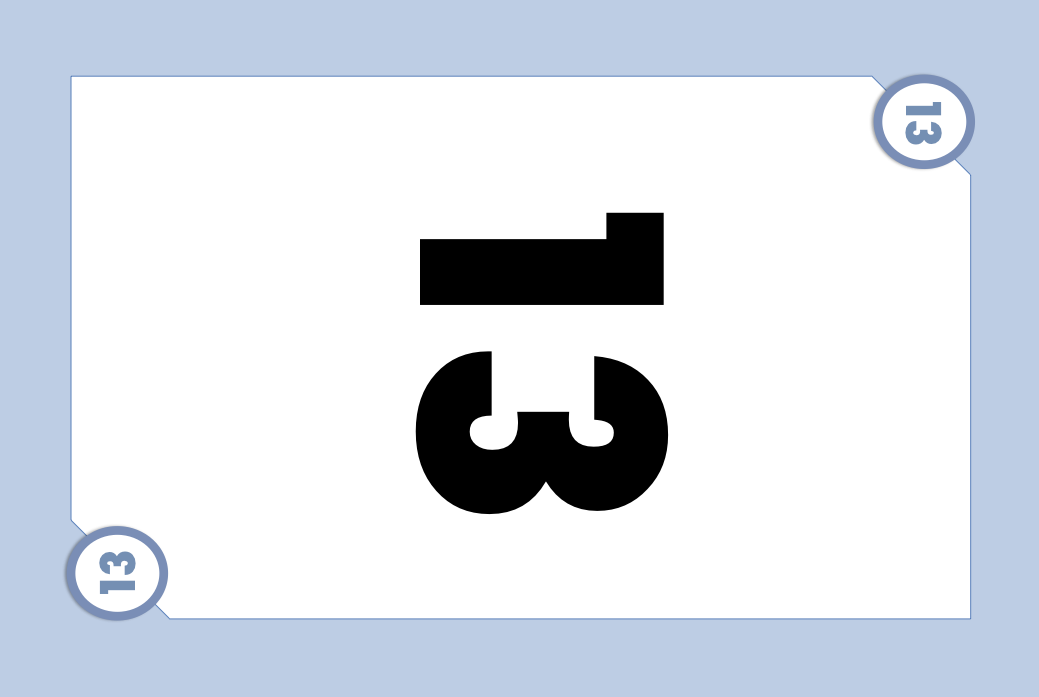
\includegraphics[angle=90,scale=\scale]{img/side-A/b-13}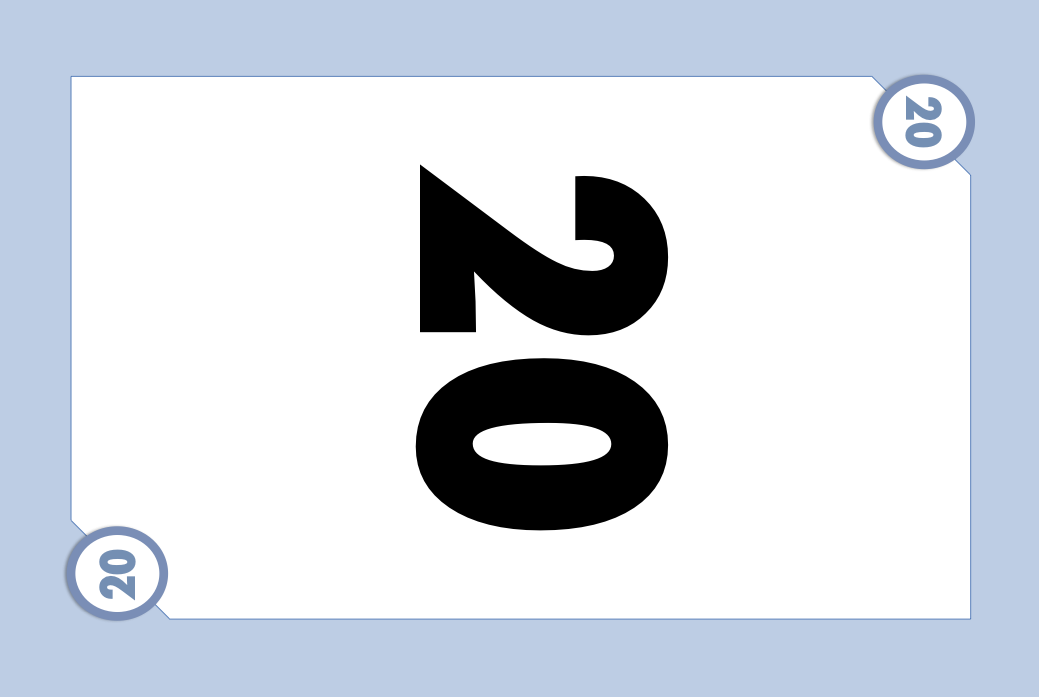
\includegraphics[angle=90,scale=\scale]{img/side-A/b-20}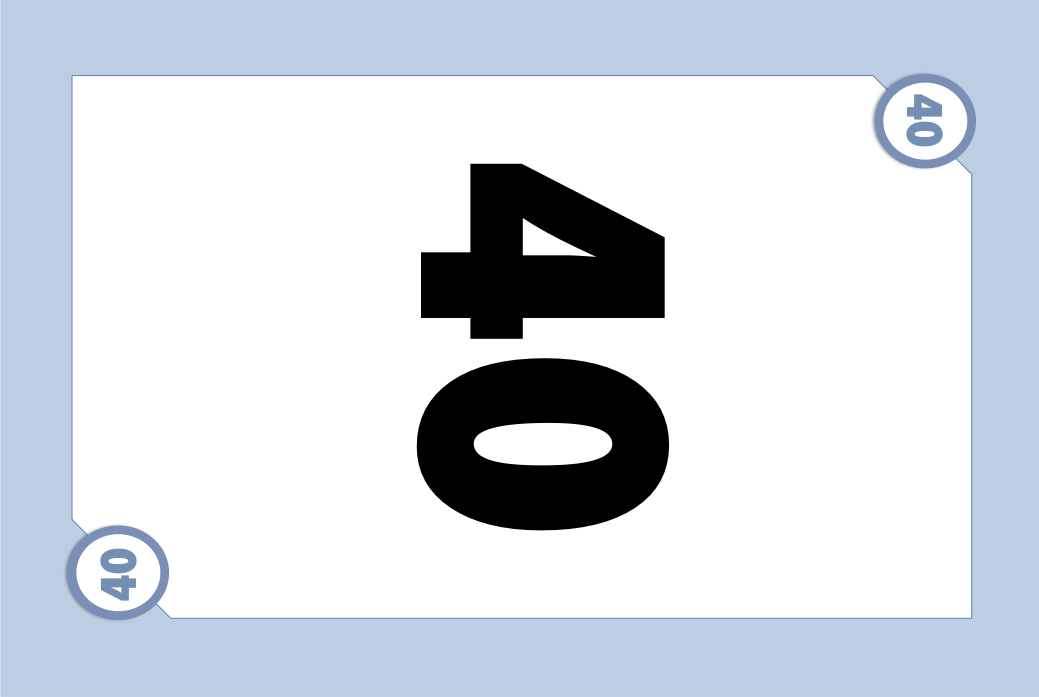
\includegraphics[angle=90,scale=\scale]{img/side-A/b-40}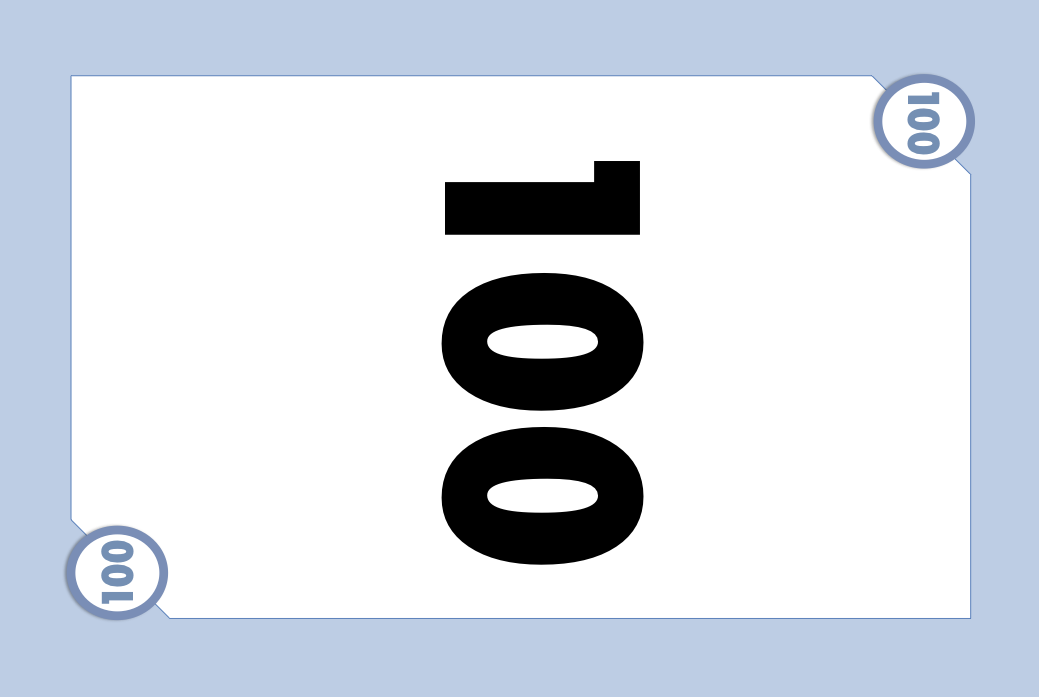
\includegraphics[angle=90,scale=\scale]{img/side-A/b-100}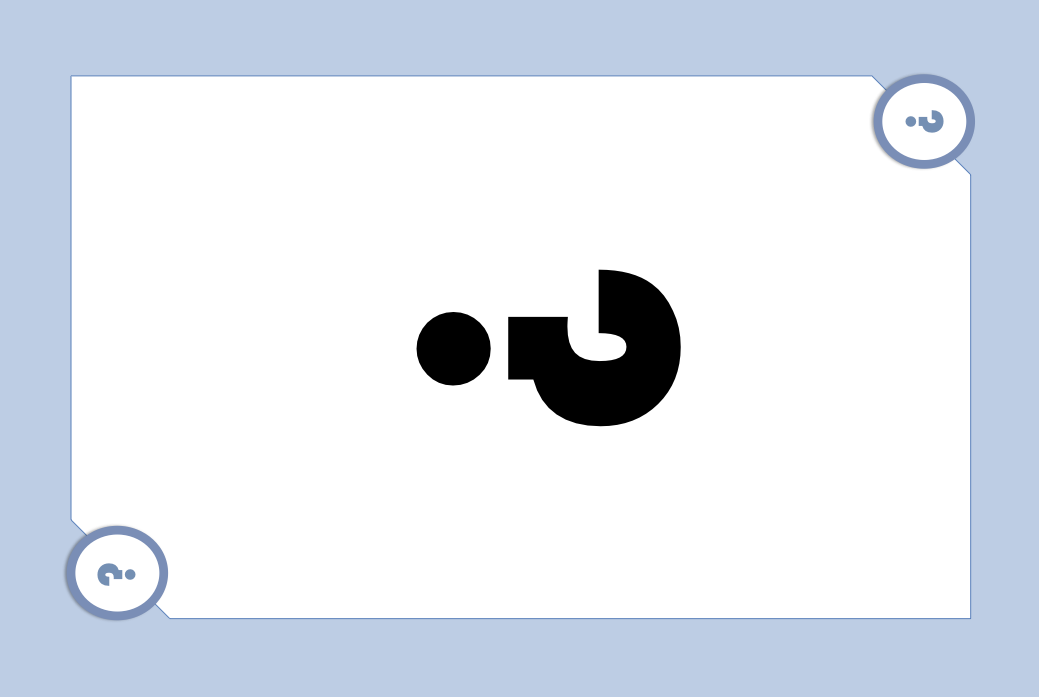
\includegraphics[angle=90,scale=\scale]{img/side-A/b-noidea}
\includegraphics[angle=90,scale=\scale]{img/side-A/b-coffee}
        \par\end{centering}
    \end{figure}
    
  \end{exampleblock}

\end{frame}

\subsection{The meeting}
\begin{frame}{The meeting}

  \begin{block}{Round 1}

    \begin{enumerate}
    \item The product owner reads a agile user story (2 minutes).
    \item The estimators discuss the feature, asking questions of the product owner as needed.
    \item Each of the members choose an estimation card.
    \item All cards are then revealed at the same time.
  \end{enumerate}    
\end{block}

\end{frame}

\begin{frame}{The meeting}

  \begin{block}{Round 2 - n}
    \begin{enumerate}
      \setcounter{enumi}{5}
    \item If all estimators selected the same value, that becomes the estimate. 
    \item If estimations diverge, the high and low estimators expose their reasons.
    \item A few minutes for the team to discuss about the story and the estimation.
    \item Again, each estimator reselects a card and all cards are again revealed at the same time.
    \end{enumerate}    
    
  \end{block}
  
\end{frame}

\begin{frame}{The meeting}
  
  \begin{block}{Taking a decision}
    
    \begin{itemize}
    \item The Planning Poker process is repeated until consensus is achieved 
    \item But, in case the estimations don’t converge by the 3rd round, there are some options:
    \begin{itemize}

    \item Left the user story apart and try again later.
    \item Ask the user to decompose the story in smaller parts.
    \item Take the highest, lowest or average estimation.
    \end{itemize}

    \end{itemize}    
  \end{block}
  
\end{frame}

\subsection{Examples}

\begin{frame}{Example}
  \def \scale{0.04}

  \begin{exampleblock}{Round 1}
    
    \begin{figure}
      \begin{centering}
        
\includegraphics[angle=90,scale=\scale]{img/side-A/b-2}
\includegraphics[angle=90,scale=\scale]{img/side-A/b-3}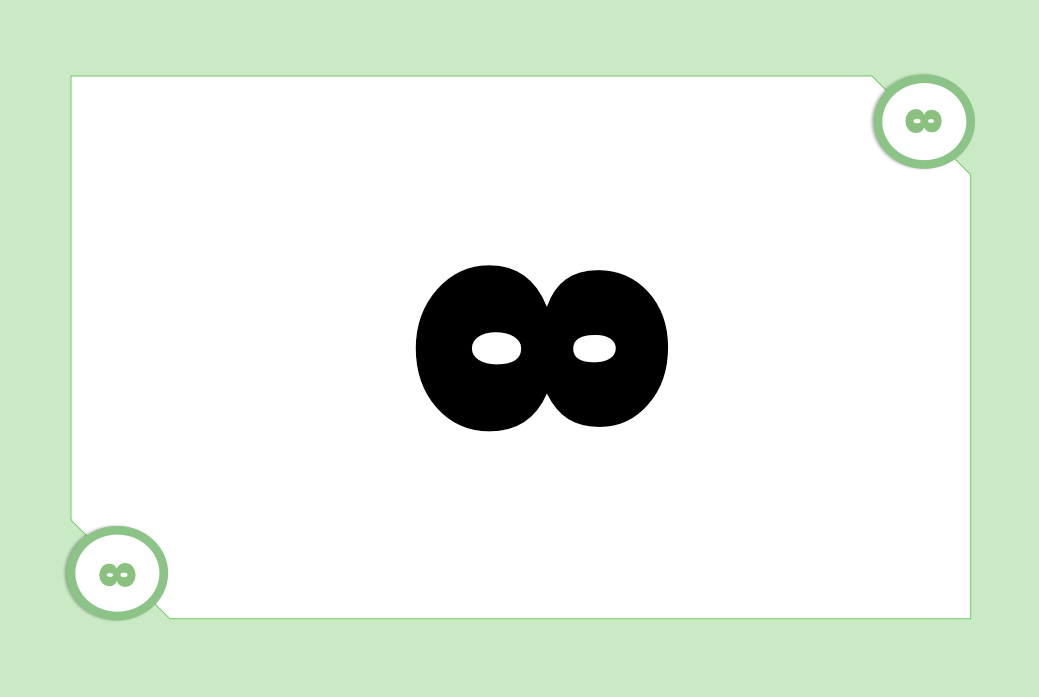
\includegraphics[angle=90,scale=\scale]{img/side-A/g-8}
\includegraphics[angle=90,scale=\scale]{img/side-A/b-3}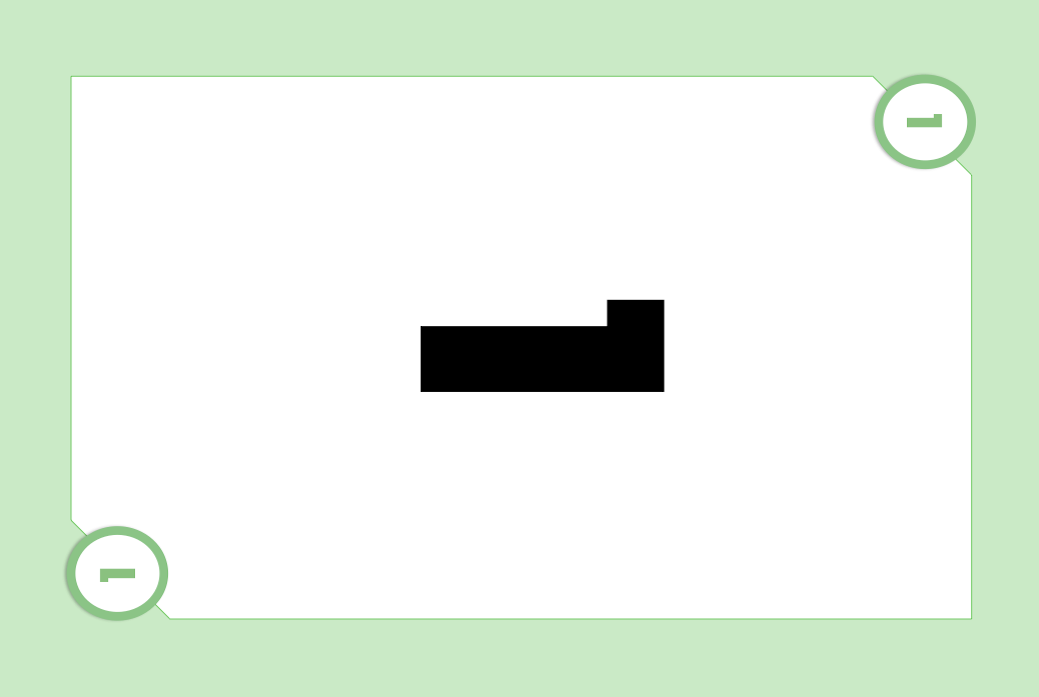
\includegraphics[angle=90,scale=\scale]{img/side-A/g-1}
        \par\end{centering}
      
    \end{figure}
    
  \end{exampleblock}
  
  \begin{exampleblock}{Round 2}
    
    \begin{figure}
      \begin{centering}
        
\includegraphics[angle=90,scale=\scale]{img/side-A/b-3}
\includegraphics[angle=90,scale=\scale]{img/side-A/b-3}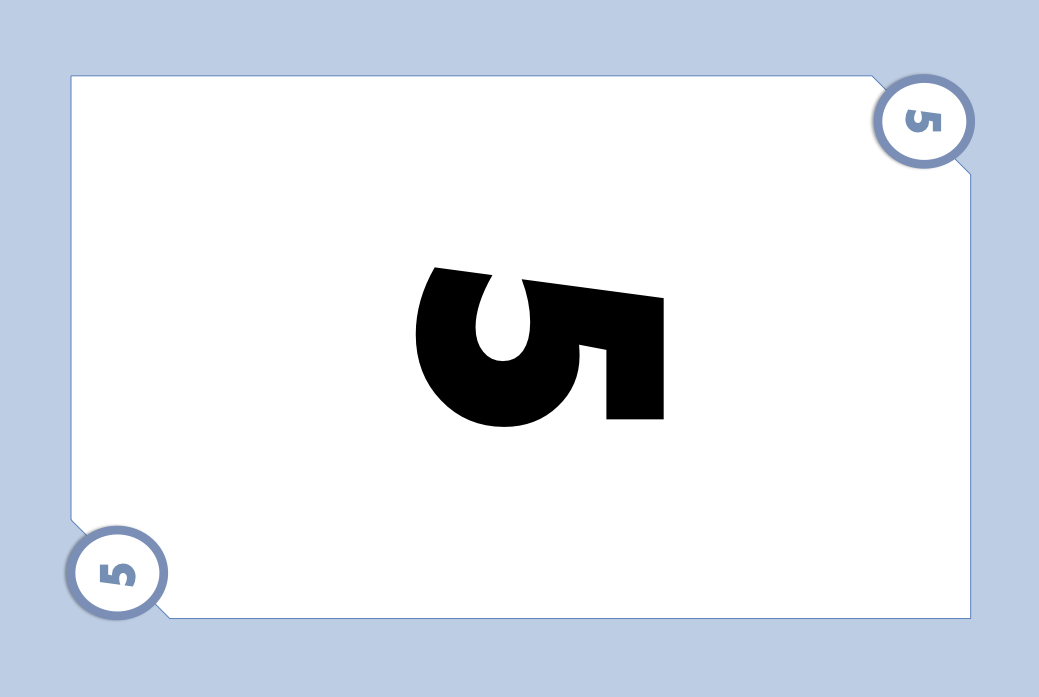
\includegraphics[angle=90,scale=\scale]{img/side-A/b-5}
\includegraphics[angle=90,scale=\scale]{img/side-A/b-3}
\includegraphics[angle=90,scale=\scale]{img/side-A/b-2}
        \par\end{centering}
      
    \end{figure}
    
  \end{exampleblock}

  \begin{block}{Solution}
    Start round 3 or take 3 or 5 as the estimation.  
  \end{block}
  
\end{frame}

\begin{frame}{Some tools}
  
  \begin{exampleblock}{Online software}
    \url{http://www.planningpoker.com/}
  \end{exampleblock}

  \begin{exampleblock}{Mobile Apps}
    \burl{https://itunes.apple.com/en/app/centare-planning-poker/id490139619?mt=8}
    
    \burl{https://play.google.com/store/apps/details?id=com.centare.PlanningPoker&hl=en}

  \end{exampleblock}
  
\end{frame}

\subsection{Advantages vs Disadvantages}

\begin{frame}{Advantages vs Disadvantages}
  
  \begin{columns}[t]  
    
    \column{.50\textwidth}
    \begin{exampleblock}{Advantages}
      \begin{enumerate}
      \item Avoid anchoring effect.
      \item Multiple expert opinions.
      \item Planning poker results in more accurate estimations.
      \item Encourages creativity, competitive spirit.
      \end{enumerate}    
    \end{exampleblock}
    
    \column{.50\textwidth}
    \begin{alertblock}{Disadvantages}
      \begin{enumerate}
      \item Meetings with the whole team are expensive.
      \item The duration of the meeting must be controlled.
      \item Interference in the estimations.
      \item Polarized estimations.
      \end{enumerate}    
    \end{alertblock}
    
    
  \end{columns}
\end{frame}

\section{Conclusion}


\begin{frame}{Conclusion}
  
  \begin{enumerate}
  \item Agile Planning Poker is a quick, simple way to estimate the Effort required to complete your Agile Stories, if carried out correctly. 
  \item Creates consensus estimate rather than having a single person driving the estimate
\item Exposes issues early through discussion of each user story
  \end{enumerate}    
  
\end{frame}

% 
% Questions
% 
\begin{frame}{}
  \begin{figure}
    \begin{centering}
      
\includegraphics[scale=0.1]{img/Icon-round-Question_mark.eps}
      \par\end{centering}
  \end{figure}
\end{frame}

% 
% Thank you
% 
\begin{frame}{}
  
  \centering {\calligra \Huge Thank you!}
  
\end{frame}

% 
% Referneces
% 

\section{References}

\begin{frame}
  
  \begin{thebibliography}{2}  
    
    \beamertemplatebookbibitems %livro
  \bibitem{Cohn}Cohn, Mike 
    \newblock \emph{Agile estimating and planning}. Pearson, 2006.
    
    \beamertemplatearticlebibitems   
    
  \bibitem{MGS}Cohn, Mike 
    \newblock  \emph{Planning Poker}
    \newblock  \url{http://www.mountaingoatsoftware.com}
    
  \bibitem{MGS}Hartman, Bob
    \newblock  \emph{An Introduction to Planning Poker}
    \newblock  \url{agile.dzone.com/articles/introduction-planning-poker}

  \bibitem{WIKI} Wikipedia
    \newblock \emph{Planning poker}.
    \newblock  \url{wikipedia.org/wiki/Planning_poker}
    
    
    \beamertemplatearticlebibitems   
    
    

  \end{thebibliography}  
\end{frame}

\end{document}

